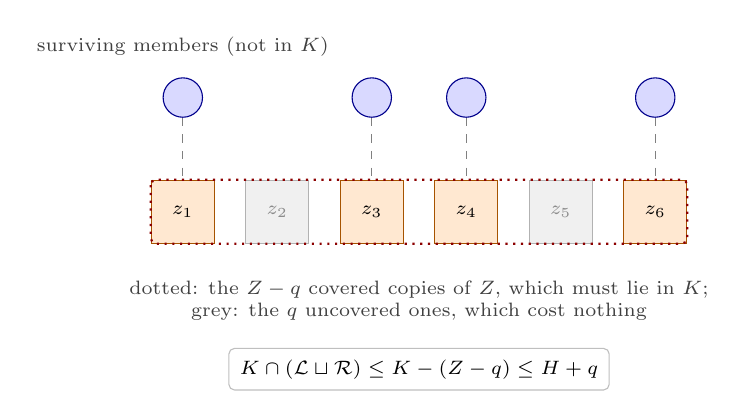
\begin{tikzpicture}[
  zv/.style={rectangle,draw=orange!65!black,fill=orange!18,minimum width=8mm,minimum height=8mm,inner sep=0pt,font=\scriptsize},
  unc/.style={rectangle,draw=black!30,fill=black!6,minimum width=8mm,minimum height=8mm,inner sep=0pt,
              font=\scriptsize,text=black!45},
  mem/.style={circle,draw=blue!55!black,fill=blue!15,minimum size=5mm,inner sep=0pt},
  cov/.style={draw=black!50,dashed},
  lab/.style={font=\scriptsize,text=black!75}
]
\node[zv]  (z1) at (0.0,0) {$z_1$};
\node[unc] (z2) at (1.2,0) {$z_2$};
\node[zv]  (z3) at (2.4,0) {$z_3$};
\node[zv]  (z4) at (3.6,0) {$z_4$};
\node[unc] (z5) at (4.8,0) {$z_5$};
\node[zv]  (z6) at (6.0,0) {$z_6$};
\node[mem] (m1) at (0.0,1.45) {};
\node[mem] (m3) at (2.4,1.45) {};
\node[mem] (m4) at (3.6,1.45) {};
\node[mem] (m6) at (6.0,1.45) {};
\foreach \a/\b in {m1/z1,m3/z3,m4/z4,m6/z6}{ \draw[cov] (\a) -- (\b); }
\draw[red!55!black,dotted,thick,rounded corners=2pt] (z1.north west) rectangle (z6.south east);
\node[lab,anchor=south] at (0.0,1.85) {surviving members (not in $K$)};
\node[lab,anchor=north,align=center] at (3.0,-0.75)
  {dotted: the $\abs Z-q$ covered copies of $Z$, which must lie in $K$;\\
   grey: the $q$ uncovered ones, which cost nothing};
\node[draw=black!25,fill=white,rounded corners=2pt,inner sep=4pt,font=\scriptsize]
  at (3.0,-2.0) {$\abs{K\cap(\mathcal L\sqcup\mathcal R)}\le\abs K-(\abs Z-q)\le\abs H+q$};
\end{tikzpicture}
